\documentclass[11pt]{article}    
\usepackage[a4paper,left=1in,right=1in,top=1in,bottom=1in]{geometry} 

\usepackage[english]{babel}
\usepackage[T1]{fontenc} 
\usepackage[utf8]{inputenc}
\usepackage{seqsplit}

\renewcommand{\familydefault}{\sfdefault} 
\usepackage{setspace}  \singlespacing  
\usepackage{graphicx}        
\usepackage[absolute]{textpos}
\usepackage{xcolor}
\usepackage{fontawesome5}
\usepackage{multirow}
\usepackage{hyperref}
\hypersetup{
    colorlinks,
    linkcolor={red!50!black},
    citecolor={blue!50!black},
    urlcolor={blue}
}

% Additional packages for the content
\usepackage{float}
\usepackage{subfig,wrapfig}
\usepackage{amsmath,amsfonts,amsthm,amssymb}
\usepackage{fancyhdr,fancybox,color}
\usepackage{enumerate}
\usepackage[amssymb]{SIunits}
\definecolor{MyBlue}{rgb}{0,0.3,0.6}
\usepackage[all]{hypcap}
\usepackage{csquotes}
\usepackage[url=false,
backend=bibtex,
style=authoryear-comp,
doi=true,
isbn=true,
backref=false,
dashed=false,
maxcitenames=2,
maxbibnames=99,
natbib=true]{biblatex}
\DeclareNameAlias{author}{family-given}
\renewbibmacro{in:}{}
\addbibresource{../_logosAndRef/references.bib}
\nonfrenchspacing

% Configurable separation between header and body
\newlength{\headertobodysep}
\setlength{\headertobodysep}{1cm}

% Header with logos and contact information
\begin{document}
\thispagestyle{empty}

% Lean header with aligned elements
\textblockorigin{0pt}{0pt}

% Durham logo on the left
\begin{textblock*}{5cm}(0.5cm,1cm)
    
\includegraphics[height=2cm]{../_logosAndRef/Durham-University.pdf}
\end{textblock*}

% Contact information in the center - vertically centered with logos
\begin{textblock*}{9cm}(6cm,1.5cm)
    \centering
    {\large \textbf{Gravity-defying liquids | CoMPhy Lab}}\\[0.2em]
    Department of Physics, Durham University\\[0.3em]
    \href{https://comphy-lab.org}{comphy-lab.org}
\end{textblock*}

% CoMPhy logo aligned with right margin
\begin{textblock*}{5cm}(15.5cm,1cm) % exactly 1 cm away from the right edge
    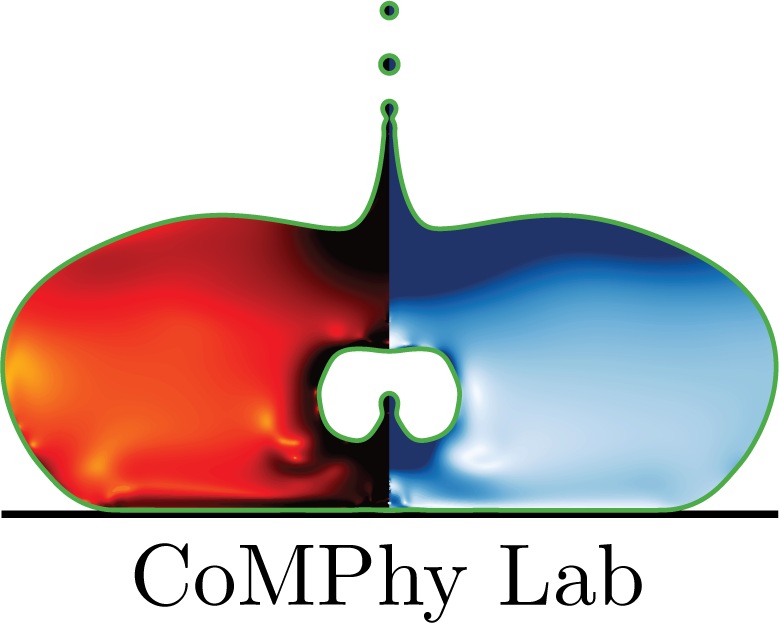
\includegraphics[height=2cm]{../_logosAndRef/CoMPhy-Lab.png}
\end{textblock*}

% Reset to normal text flow after header
\vspace*{\headertobodysep}

\begin{center}
    \begin{LARGE}
     Gravity-defying liquids
    \end{LARGE}
\end{center}

\section*{Description}
Viscoplastic/yield-stress fluids are commonly observed in our daily life, like toothpaste, ketchup, and hair gel, which unlike Newtonian liquids, do not flow under the influence of gravity when inverted. A new class of yield-stress fluids is thermoresponsive viscoplastic gels, which are frequently used in inkjet printing applications. These gels show viscoplastic shear-thinning behavior at low temperatures due to the presence of a gel network. However, at high temperatures, the gel network dissolves, and the liquid shows Newtonian behavior. In this project, we aim to understand what happens when a droplet of such liquid impacts on a flat, horizontal substrate (Figure~\ref{Fig::Fig1}(a)). The droplet is initially at a high temperature exhibiting Newtonian behavior. However, when it impacts a substrate at low temperature, the gel network starts to form, and viscoplastic behavior is observed (Figure~\ref{Fig::Fig1}(b)). Furthermore, as the droplet recoils back, a clear distinction between a Newtonian and a high yield stress drop can be observed (Figure~\ref{Fig::Fig1}(c)). For this work, we will use Direct Numerical Simulations of the drop impact of yield stress fluids. One of the deliverables will be to understand the effect of yield stress and shear thinning behavior on the droplet's post-impact morphology. The work is part of an academic-industrial collaboration and provides the opportunity to study interesting, complex physics and solve real-world problems. 
\begin{figure}[H]
 \begin{center}
  \includegraphics[width= 0.65\textwidth]{ProposalPicture.eps}
 \end{center}
 \caption{Yield stress drop impact on solid substrate.}
 \label{Fig::Fig1}
\end{figure}

\section*{What you will do and what you will learn?}
In the Physics of Fluids group, we are looking for enthusiastic students to join our newly established project on thermoresponsive gels. 
\begin{enumerate}
	\item You will learn about rheology of complex non-Newtonian fluids. 
	\item You will work with experimentalists and our industrial collaborators at Canon printing company.
	\item You will learn about the Computational Fluid Dynamics (CFD) fundamentals, and use the free software program Basilisk C \href{http://basilisk.dalembert.upmc.fr}{(http://basilisk.dalembert.upmc.fr)}. 
	\item You will learn how to do basic and advanced scientific data analysis. 
	\item As a part of the \href{https://comphy-lab.org}{CoMPhy lab} at the Physics of Fluids Dept., you will learn and adapt open-source coding principles. 
\end{enumerate}

If you have any questions, feel free to contact us \href{mailto:vatsal.sanjay@comphy-lab.org}{vatsal.sanjay@comphy-lab.org}/\href{mailto:vatsal.sanjay@durham.ac.uk}{vatsal.sanjay@durham.ac.uk} or drop by Ph255 at the Department of Physics at Durham University.
\begin{center}
\begin{tabular}{|l|l|l|}
\hline \textbf{Collaborators} & \textbf{E-mail} & \textbf{Based at} \\
\hline Dr. Vatsal Sanjay & \href{mailto:vatsal.sanjay@comphy-lab.org}{vatsal.sanjay@comphy-lab.org} & Ph255 (Rochester building) \\
\hline Ayush Dixit & \href{mailto:a.k.dixit@utwente.nl}{a.k.dixit@utwente.nl} & Univ. Twente \\
\hline Prof. Dr. Detlef Lohse & \href{mailto:d.lohse@utwente.nl}{d.lohse@utwente.nl} & Univ. Twente  \\
\hline
\end{tabular}
\end{center}

\vspace{1em}
\noindent\textit{Last updated: \today}

\printbibliography
\end{document}